\chapter{Advanced Tutorial}
This chapter is a small introduction of using advanced \LaTeX-commands with examples. Enjoy! We recommend to use the Overleaf tutorial to get the first experience with \LaTeX\footnote{\url{https://www.overleaf.com/learn/latex/Learn_LaTeX_in_30_minutes}}. 
\newpage
%%%%%%%%%%%%%%%%%%%%%%%%%%%%%%%%%%%%%%%%%%%%%%%%%%%
\section{Code Listings}
If there is some interesting code you would like to show
in order to ease the understanding of the text,
you can just include it using the \verb+lstlisting+ environment.
Have a look at the source of this page to see how this is included:

\begin{lstlisting}[language=Go]
x := from(42);
\end{lstlisting}

You could also put the code into an external file
and include it in this document using the \verb+lstinputlisting+ command:

\lstinputlisting[language=Go]{listings/example.go}

Be careful not to include large files as it hampers readability.
If there is a short excerpt from a large file you would like to show,
you can also extract an explicit range of lines from it without the need to modify the source file.
This next listing only shows the conditional from the previous code:

\lstinputlisting[language=Go, firstline=2, lastline=5, firstnumber=1, caption={Example of including code segments from file}]{listings/example.go}

To use more advanced syntax highlighting
have a look at the available options of the \emph{listings} package
or use the \emph{minted} package\footnote{\url{https://texdoc.net/texmf-dist/doc/latex/minted/minted.pdf}},
which has more extensive language support and additional themes.
Both can be configured in the main file.
%%%%%%%%%%%%%%%%%%%%%%%%%%%%%%%%%%%%%%%%%%%%%%%%%%%
\newpage
\section{Math}
In case you need to include some math,
the \emph{amsmath} package\footnote{\url{https://texdoc.net/texmf-dist/doc/latex/amsmath/amsmath.pdf}} is already included in this document.

To properly display some short formula like \( e^{i \pi} = -1\),
you can use the \verb+\( \)+ inline command.
For larger formulas, the \verb+math+ environment is more appropriate.
If you need to reference the formula multiple times,
e.g. in case it is used in theorems,
you should use the \verb+equation+ environment:

\begin{equation}
	\vec\nabla\times\vec{B}= \mu_0\vec{j}+\mu_0\varepsilon_0\frac{\partial\vec{E}}{\partial t}
	\label{func}
\end{equation}

To reference it as~\eqref{func} using the \verb+\eqref{}+ command,
remember to use a \verb+\label{}+.
%%%%%%%%%%%%%%%%%%%%%%%%%%%%%%%%%%%%%%%%%%%%%%%%%%%%
\section{Including figures}
%%%
\begin{figure}[ht]    \centering
    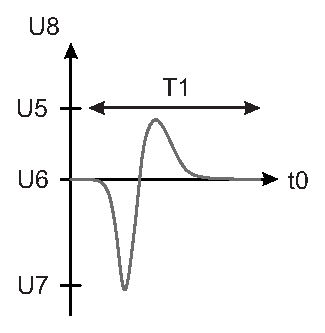
\includegraphics[width=0.35\textwidth]{figures/example.eps}
    \caption{Timing of an extracellular spike waveform recorded from the MEA}
    \label{fig:NeuronSetup0}
\end{figure}
%%%
Including jpg and png are only possible with pdflatex as compiler. Otherwise only eps can be used.

%%%%%%%%%%%%%%%%%%%%%%%%%%%%%%%%%%%%%%%%%%%%%%%%%%%%
\newpage
\section{Change text in vector graphics}
You can change the text content of a text string in a vector graphic by using the \verb+\psfrag{}[][]{}+ command in order to achieve a similar design.
%%%
\begin{figure}[ht]  \centering
    \psfrag{t0}[l][l]{$t$}
    \psfrag{T1}[c][c]{$T_{sp}$}
    \psfrag{U0}[l][l]{$U_{int}(t)$}
    \psfrag{U5}[r][r]{$\SI{100}{\micro V}$}
    \psfrag{U6}[r][r]{$\SI{0}{\micro V}$}
    \psfrag{U7}[r][r]{$\SI{-200}{\micro V}$}
    \psfrag{U8}[c][c]{$U_{ext}(t)$}
    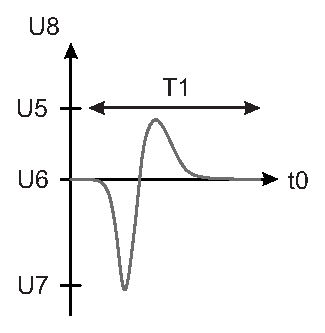
\includegraphics[width=0.25\textwidth]{figures/example.eps}
    \label{fig:TutorialNeuron1}
\end{figure}
%%%
For using it in Overleaf, you have to change the compiler from \verb+pdflatex+ to LaTeX. Otherwise it will not work!

You can also create figures with several subfigures/subfloats.
%%%
\begin{figure}[ht]    \centering
    \subfloat[]{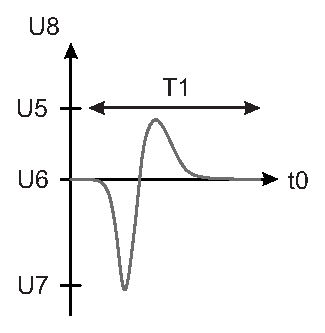
\includegraphics[width=0.25\textwidth]{figures/example.eps}} \hspace{5mm}
    \subfloat[]{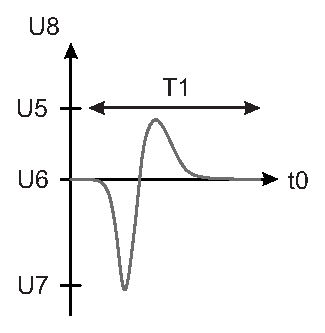
\includegraphics[width=0.25\textwidth]{figures/example.eps}}
    \caption{Timing of an extracellular spike waveform recorded from the MEA}
    \label{fig:TutorialNeuron2}
\end{figure}
%%%
With the command \verb+\hspace+, you can control the horizontal space between the several figures. Otherwise, they will be connected directly. An alternativ command is \verb+\hfill+ in which the distance between the figures is automated set in order to have the figures at the outer corner. 
%%%%%%%%%%%%%%%%%%%%%%%%%%%%%%%%%%%%%%%%%%%%%%%%%%%%
\newpage
\section{Create Timing Diagram}
Using the \verb+tikz+-Package for creating timing diagram of digital circuits.\\

\begin{figure}[ht]
    \begin{tikztimingtable}
        System states                     & 1D{} [fill=yellow]4D{Samp.} 25D{Conv.} 4D{NS} [fill=white]3D{Idle}\\
        Chopping clock $f_{ch}$           & 7L 30H  \\
        Sampling clock $f_{s}$            & 1L 1H 35L \\
        Input sampling $\Phi_{smp}$       & 2L 3H 32L \\
        Conversion clock $\Phi_{cnv}$     & 6L 24{C} 7L \\
        Selection signals $\Phi_{sl}(x)$  & 6L 24H 7L \\
        Data SAR $\Phi_{D,x}$             & 6L 2D{11} 2D{10} 2D{9} 2D{8} 2D{7} 2D{6} 2D{5} 2D{4} 2D{3} 2D{2} 2D{1} 2D{0} 7L \\
        Residual sampling $\Phi_{sh}$     & 30L 2H 5L \\
        Residual integration $\Phi_{int}$ & 32L 2H 3L \\
        End of conversion $\Phi_{EOC}$    & 1H 33L 3H  \\
        \extracode
        \begin{pgfonlayer}{background}
        \vertlines[help lines, gray]{1,5,30,34}
        \end{pgfonlayer}
        % \tablegrid[fill=red,green!25,step=1]
    \end{tikztimingtable}
    \caption[Timing diagram of the Successive Approximation Analog-Digital Converter]{Timing diagram of the Successive Approximation Analog-Digital Converter (SAR ADC) control with noise shaping of the residual voltage~$\Delta U$ after each conversion step} 
    \label{fig:TimingSAR}
\end{figure}
%%%
%%%%%%%%%%%%%%%%%%%%%%%%%%%%%%%%%%%%%%%%%%%%%%%%%%%%
\newpage
\section{Create Circuit Diagrams}
With the \verb+circuitikz+ environment, you can create circuit diagram of electronic circuit diagrams. For creating these circuit diagrams, the website \url{https://circuit2tikz.tf.fau.de/designer} helps to create these easily. They can be imported and exported in *.svg and *.tex.
%%%
\begin{figure}[ht] \centering
    \begin{circuitikz}
    \node [op amp, noinv input up](OP1){OTA};
    \draw (OP1.+) to[resistor, R=$R_i$] ++(-2,0) to[vsource, v=$U_0$] ++(0,-3) node[ground](){}
    ;
    \draw (OP1.out) to[R=$R_{out}$] ++(1.5,0) node[nfet, anchor=G](T1){};
    \draw (T1.S) to[short, i=$i_L$] ++(0,-0.6) coordinate(FB) to[resistor, R=$R_s$] ++(0,-1.5) node[ground]{}
    ;
    \draw (T1.D) to[leD, mirror, invert] ++(0,1.5) node[vcc](vcc){$V_{DD}$}
    ;
    \draw (OP1.-) to[short] ++(0,-0.9) to[short,-*] (FB)
    ;
    \draw (FB) to[short] ++(2,0) to[C, C=$C_s$] ++(0,-1.5) node[ground]{}
    ;
    \end{circuitikz}
    \caption{Circuit diagram of a voltage-controlled current driver circuit for LEDs}
    \label{fig:Filter1}
\end{figure}
%%%%%%%%%%%%%%%%%%%%%%%%%%%%%%%%%%%%%%%%%%%%%%%%%%%%
\section{Data visualisation with Python}
Often you have to visualize the data of your experiment in order to explain the results rightful and easily. For this, the online handbook\footnote{\url{https://www.oreilly.com/library/view/python-data-science/9781491912126/ch04.html}} for data visualisation in Python can help you to get the right plots by using \verb+Matplotlib+ package.
%%%%%%%%%%%%%%%%%%%%%%%%%%%%%%%%%%%%%%%%%%%%%%%%%%%%
\newpage
\section{Table}
Generate nice tables with the following example with command \verb+definecolor+ for defining and \verb+rowcolor+ for setting by using the package \verb+colortbl+.
%%%
\begin{table*}[ht]    \centering
    \definecolor{lavender}{rgb}{0.89, 0.89, 0.89}
    \caption{Overview of different implementations of neural decoding for the movement intention using spikes}
    \begin{tabular}{lm{4cm}lm{3cm}m{3cm}} \hline 
        \textbf{Year}   & \textbf{Decoding Objective} & \textbf{Primate} & \textbf{Architecture} & \textbf{Methods Comparing} \\ \hline\hline 
        \rowcolor{lavender}
        2012   & Cursor movement prediction on the screen & NHP & ESN (RNN~variant) & VKF \\
        2018 & Reach Kinematics & NHP, Human & LFADS (RNN~variant) & GPFA \\ 
        \rowcolor{lavender}
        2018        & Hindlimb Kinematics & NHP & LSTM  & WF, PLDS+WF, XGBoost, RNN \\ 
        2018      & Reach Kinematics & NHP & rEFH (RBM~variant) & WF, KF, UKF \\
        \rowcolor{lavender}
        2018  & Wrist EMG & NHP &  AE+ADAN & CCA, KLDM \\
        2019      & Wrist EMG & NHP & LSTM  & WF, WC\\  
        \rowcolor{lavender}
        2019        & Reach Kinematics& NHP & LSTM & KF\\ 
        2019      & Reach and Hindlimb Movement & NHP & Multilayer LSTM  & WF, KF, UKF, LSTM\\ 
        \rowcolor{lavender}
        2020     & Reach Kinematics & NHP & LSTM  & WF, WC, KF, NB, SVR, XGB, FNN, RNN, GRU, Ensemble\\ 
        2021     & Reach Kinematics & NHP & Quasi-RNN  & WF, WC, KF, UKF, SRNN, GRU, LSTM  
        \\ \hline
    \end{tabular} 
    \label{tab:ND}
\end{table*}
%%%
%%%%%%%%%%%%%%%%%%%%%%%%%%%%%%%%%%%%%%%%%%%%%%%%%%%%
\section{Citation}
If you have some information from other source like scientific papers, please mention this. This \LaTeX-document uses \verb+biblatex+. The file libary.bib includes all papers which you can load via \verb+\cite{}+ and use the following declaration \{Author+Year\}. If you use it, then use \verb+\cite{Lee2021}+ and it appears.
\newpage
%%%%%%%%%%%%%%%%%%%%%%%%%%%%%%%%%%%%%%%%%%%%%%%%%%%%
\section{Create Tikz diagrams}
With using \verb+tikz+ package you can create several types of pictures. 

%%%%%%%%%%%%%%%%%%%%%%%%%%%%%%%%%%%%%%%%%%%%%%%%%%%%%%%%%%%%%%%%%%%%%%%%%%%%
\subsection{Flow diagram}
\tikzstyle{int}=[draw, fill=blue!20, minimum size=2em]
\tikzstyle{init} = [pin edge={to-,thin,black}]

\begin{tikzpicture}[node distance=2.5cm]
    \node [int, pin={[init]above:$v_0$}] (a) {$\frac{1}{s}$};
    \node (b) [left of=a,node distance=2cm, coordinate] {a};
    \node [int, pin={[init]above:$p_0$}] (c) [right of=a] {$\frac{1}{s}$};
    \node [coordinate] (end) [right of=c, node distance=2cm]{};
    \path[->] (b) edge node {$a$} (a);
    \path[->] (a) edge node {$v$} (c);
    \draw[->] (c) edge node {$p$} (end) ;
\end{tikzpicture}

%%%%%%%%%%%%%%%%%%%%%%%%%%%%%%%%%%%%%%%%%%%%%%%%%%%%%%%%%%%%%%%%%%%%%%%%%%%%
\subsection{System Diagram}
An example of drawing system designs ...

% Define distances for bordering
\def\blockdist{2.3}
\def\edgedist{2.5}
\begin{tikzpicture}[
    sensor/.style = {draw, fill=blue!20, text width=5em, text centered, minimum height=2.5em},
    ann/.style = {above, text width=5em, text centered},
    wa/.style = {sensor, text width=10em, fill=red!20, minimum height=6em, rounded corners},
    sc/.style = {sensor, text width=13em, fill=red!20, minimum height=10em, rounded corners}
]
    \node (wa) [wa]  {System Combination};
    \path (wa.west)+(-3.2,1.5) node (asr1) [sensor] {$ASR_1$};
    \path (wa.west)+(-3.2,0.5) node (asr2)[sensor] {$ASR_2$};
    \path (wa.west)+(-3.2,-1.0) node (dots)[ann] {$\vdots$}; 
    \path (wa.west)+(-3.2,-2.0) node (asr3)[sensor] {$ASR_N$};    
    \path (wa.east)+(\blockdist,0) node (vote) [sensor] {$\theta_0,\theta_1,...,\theta_M$\\Estimated Parameters};
    \path [draw, ->] (asr1.east) -- node [above] {} 
        (wa.160) ;
    \path [draw, ->] (asr2.east) -- node [above] {} 
        (wa.180);
    \path [draw, ->] (asr3.east) -- node [above] {} 
        (wa.200);
    \path [draw, ->] (wa.east) -- node [above] {} 
        (vote.west);             
    \path (wa.south) +(0,-\blockdist) node (asrs) {System Combination - Training};
    \begin{pgfonlayer}{background}
        \path (asr1.west |- asr1.north)+(-0.5,0.3) node (a) {};
        \path (wa.south -| wa.east)+(+0.5,-0.3) node (b) {};
        \path (vote.east |- asrs.east)+(+0.5,-0.5) node (c) {};     
        \path[fill=yellow!20,rounded corners, draw=black!50, dashed]
            (a) rectangle (c);           
        \path (asr1.north west)+(-0.2,0.2) node (a) {};       
    \end{pgfonlayer}
    
    % Validation Layer is the same except that there are a set of nodes and links which are added
    \path (wa.south)+(-2.0,-7.5) node (syscomb) [sc] {\textbf{System Combination \\Algorithm}\\Estimated Parameters\\from training};
    \path (syscomb.west)+(-2.2,1.5) node (asrt1) [sensor] {$ASR_1$};
    \path (syscomb.west)+(-2.2,0.5) node (asrt2)[sensor] {$ASR_2$};
    \path (syscomb.west)+(-2.2,-1.0) node (dots)[ann] {$\vdots$}; 
    \path (syscomb.west)+(-2.2,-2.0) node (asrt3)[sensor] {$ASR_N$};    
    \path [draw, ->] (asrt1.east) -- node [above] {} 
        (syscomb.160) ;
    \path [draw, ->] (asrt2.east) -- node [above] {} 
        (syscomb.180);
    \path [draw, ->] (asrt3.east) -- node [above] {} 
        (syscomb.200);          
    \path (wa.south) +(0,-\blockdist) node (sct) {System Combination - Training};
    \path (syscomb.east)+(1.0,0.0) node (bwtn) {};

    % Note how the single nodes are repeated using for loop
    \foreach \x in {0,1,...,4}{ 
        \draw (bwtn.east)+(\x,0) node (asr\x-2)[]{}; 
        \fill (bwtn.east)+(\x,0) circle (0.1cm); 
    }
    \path [draw, ->] (syscomb.east) -- node [above] {} 
        (bwtn.east);
	\path [draw, ->] (asr0-2) -- node [above] {@} 
        (asr1-2);
    \path [draw, -] (asr1-2) -- node [above] {b} 
        (asr2-2);
    \path [draw, -] (asr2-2) -- node [above] {z} 
        (asr3-2);
    \path [draw, -] (asr3-2) -- node [above] {} 
        (asr4-2);
    \path [draw, ->] (asr0-2) edge[bend  right]  node [below] {@} 
        (asr1-2);
    \path [draw, ->] (asr1-2) edge[bend  right]  node [below] {b} 
        (asr2-2);
    \path [draw, ->] (asr2-2) edge[bend  right]  node [below] {c} 
        (asr3-2);
    \path [draw, ->] (asr4-2) node[]{} (asr4-2)+(1.0,0);
    \begin{scope}[looseness=1.6]
        \path [draw, ->] (asr0-2) edge[bend  right=90]  node [below] {a} 
            (asr1-2);
        \path [draw, ->] (asr1-2) edge[bend  right=90]  node [below] {b} 
            (asr2-2);
        \path [draw, ->] (asr2-2) edge[bend  right=90]  node [below] {c} 
            (asr3-2);
    \end{scope}
    \path (asr3-2.east)+(1.5,0.0) node (bw)[sensor] {Best Word Sequence\\$\arg\max$};    
    \path [draw, -] (asr1-2.east) node [below] {} 
        (bw.west);       
    \begin{pgfonlayer}{background}
        \path (asrt1.west)+(-0.5,1.0) node (g) {};
        \path (bw.east |- syscomb.south)+(0.5,-1.5) node (h) {};
         
        \path[fill=yellow!20,rounded corners, draw=black!50, dashed]
            (g) rectangle (h);

        \path [draw, ->] (vote.south) edge[bend  left=90]  node [below] {Used in validation} 
            (syscomb.30);            
    \end{pgfonlayer}
    \path (asr1-2.south) +(-\blockdist,-\blockdist) 
        node (asrs) {System Combination - Validation};
\end{tikzpicture}

%%%%%%%%%%%%%%%%%%%%%%%%%%%%%%%%%%%%%%%%%%%%%%%%%%%%%%%%%%%%%%%%%%%%%%%%%%%%
\subsection{Deep Neural Networks}
This first example shows the functionality to plot a deep neural network with half-automated settings.
\begin{figure}[h]  \centering
    \def\hspacelayer{3.5cm}
    \def\vspacelayer{0.1cm}
    \def\posweights{0.16}
    \def\inputsizeB{2}
    \def\hiddensizeBA{1}
    \def\hiddensizeBB{1}
    \def\outputsizeB{1}
    \begin{tikzpicture}[
        scale=1.05,
        shorten >=1pt,->,draw=black!70, node distance=\vspacelayer,
        % Weights and bias of NN
        edge/.style 2 args={pos=\posweights, above, sloped, font=\small},
        weight/.style 2 args={
            edge={#1}{#2}, fill=white, inner sep=2pt, 
            node contents={\pgfmathparse{0.35*#1-#2*0.15+0.05}\pgfmathprintnumber[fixed]{\pgfmathresult}}
        }        
      ]
    % --- Definition of neurons
    \foreach \y in {0,...,\inputsizeB}
        \pgfmathparse{(1 - \y - 0.5 * mod(\inputsizeB, 2)) * \vspacelayer}
        \node[input neuron] (i\y) at (0* \hspacelayer,  \pgfmathresult) {$x_\y$};
    \foreach \y in {0,...,\hiddensizeBA}
        \pgfmathparse{(1 - \y - 0.5 * mod(\hiddensizeBA, 2)) * \vspacelayer}
        \path node[hidden neuron] (h0\y) at (1* \hspacelayer, \pgfmathresult) {$h_{0,\y}$};
    \foreach \y in {0,...,\hiddensizeBB}
        \pgfmathparse{(1 - \y - 0.5 * mod(\hiddensizeBB, 2)) * \vspacelayer}
        \path node[hidden neuron] (h1\y) at (2* \hspacelayer, \pgfmathresult) {$h_{1,\y}$};
    \foreach \y in {0,...,\outputsizeB}
        \pgfmathparse{(1 - \y - 0.5 * mod(\outputsizeB, 2)) * \vspacelayer}
        \node[output neuron] (o\y) at (3* \hspacelayer, \pgfmathresult) {$y_\y$};
    % --- Adding text with layer name
    \foreach \name [count=\x from 0] in {Input layer, Hidden layer \#1, Hidden layer \#2,  Output layer}
        \node[annot] (text node1) at (\x* \hspacelayer, -4) {\name};
    % --- Drawing lines (Connect every node of one layer to the next layer)
    \foreach \source in {0,...,\inputsizeB}
        \foreach \dest in {0,...,\hiddensizeBA}
            \path (i\source) edge (h0\dest);
    \foreach \source in {0,...,\hiddensizeBA}
        \foreach \dest in {0,...,\hiddensizeBB}
            \path (h0\source) edge (h1\dest);
    \foreach \source in {0,...,\hiddensizeBB}
        \foreach \dest in {0,...,\outputsizeB}
            \path (h1\source) edge (o\dest);
    % --- Drawing the weight values on lines
    \foreach \i in {0,...,\inputsizeB}
        \foreach \j in {0,...,\hiddensizeBA}
            \path (i\i) -- (h0\j) node[weight={\i}{\j}];
    \foreach \i in {0,...,\hiddensizeBA}
        \foreach \j in {0,...,\hiddensizeBB}
            \path (h0\i) -- (h1\j) node[weight={\i}{\j}];
    \foreach \i in {0,...,\hiddensizeBB}
        \foreach \j in {0,...,\outputsizeB}
            \path (h1\i) -- (o\j) node[weight={\i}{\j}];
            
    \end{tikzpicture}
    \caption{Struktur des Neuronalen Netzes}
    \label{fig:dnn_network}
\end{figure}

For more details of using layer, it is recommended to use this structure ...\\
%%%%
\begin{figure}[h]    \centering
\def\modelboxwidth{12em}
\def\modelboxheight{1.6em}
\begin{tikzpicture}[
        -{LaTeX}, thick,
        every node/.style={draw},
        layer basic/.style = {
            rectangle, 
            rounded corners,
            draw=black,
            text width=\modelboxwidth,
            minimum height=\modelboxheight, 
            text centered,
            rotate=90
        },
        layer mod/.style= {layer basic, fill=black!8, thin, font={#1}},
        layer io/.style={layer basic, fill=blue!8, thick, font={#1}}
    ]
    % --- Generate frames
    \foreach \name [count=\x from 0] in {{Frame Input (1x32)}, {Class. Output (1x4)}}
        \node (i\x) at (\x* 27.0em, 0) [layer io={\name}] {};
    \foreach \name [count=\x from 0] in {{Linear(28,16)}, BatchNorm1D, SiLU}
        \node (a\x) at (4em+\x*\modelboxheight, 0) [layer mod={nn.\name}] {};
    \foreach \name [count=\x from 0] in {{Linear(16,10)}, BatchNorm1D, Sigmoid}
        \node (b\x) at (11em+\x*\modelboxheight, 0) [layer mod={nn.\name}] {};
    \foreach \name [count=\x from 0] in {Dropout(0.1), {Linear(10,4)}, BatchNorm1D, Softmax}
        \node (c\x) at (18em+\x*\modelboxheight, 0) [layer mod={nn.\name}] {};
    % --- Generate arrow
    \draw (i0) edge (a0);
    \path (a2) edge (b0);
    \path (b2) edge (c0);
    \path (c3) edge (i1);
\end{tikzpicture}
\caption{Caption}
\label{fig:NNmodel}
\end{figure}
%%%
%%%%%%%%%%%%%%%%%%%%%%%%%%%%%%%%%%%%%%%%%%%%%%%%%%%
\newpage
\section{Creating plots}
Using the package \textit{pgfplots} in combination with \textit{tikzpicture}, you can create plots in \LaTeX. Here are two examples by using default settings for function and scatter plotting.
%%%
\subsection{Linear plots}
\begin{figure}[h] \centering
    \begin{tikzpicture}
        \begin{axis}[plot_graphs,
            domain=-3:3, xlabel={$x$}, ylabel={$f(x)$}, 
            xmin=-3, xmax=3]
            \addplot[mark=none, line width=1mm, red, domain=-3:0]{0};
            \addplot[mark=none, line width=1mm, red, domain=0:3]{x};
        \end{axis}
    \end{tikzpicture}
\end{figure}
%%%
\subsection{Scatter plots}
\begin{figure}[h]   \centering
\begin{tikzpicture}[scale=1.1]
    \begin{axis}[plot_scatter,        
        width=0.85\textwidth,
        height=10cm,
        xlabel={Feat. 2}, xmin=2, xmax=4, xtick={2,2.1,...,4},
        ylabel={Feat. 1}, ymin=550, ymax=725, ytick={550,575,...,725},
    ]
    \addplot[
        draw=white,
        only marks,
        scatter,
        scatter src=explicit symbolic,
        mark=*,
        mark size=3pt
    ]
    %table[x=x,y=y,meta=label,col sep=comma] {1_tasks/table.csv};
    table[meta=label]{figures/scattered_example.dat};
    \end{axis}
\end{tikzpicture}
\caption{Caption}
\label{fig:task_knn}
\end{figure}
\newpage
%%%%%%%%%%%%%%%%%%%%%%%%%%%%%%%%%%%%%%%%%%%%%%%%%%%
\section{Plagiarism}
Plagiarism is the appropriation of other people's intellectual achievements without labelling. This can refer to the adoption of third-party texts or other representations or ideas. Plagiarism can, but does not necessarily have to, violate the law: The adoption of third-party texts that are not labelled as quotations is generally an infringement of copyright. The use of other people's ideas can be an infringement of patent rights or design patents. In academia, plagiarism can violate examination regulations, employment contracts or university law. There is a grey area between the unlawful adoption of other people's intellectual work and the legitimate adoption of free or liberated ideas, where plagiarism is considered legal but not legitimate.

Just to make sure that your thesis does not contain a plagiarism, you can check it with Grammarly\footnote{\url{https://www.grammarly.com/}} or other tools. If you want to copy the idea or the results of a paper or patent, then rewrite the text with your own words.

If your thesis contains a plagiarism, then it will be carefully checked by the examination board and they will make a decision. In the worst case, this means a fine of up to 50,000~€ and the immediate end of your studies.